\documentclass[11pt,letterpaper]{article}

\usepackage[margin=0.85in]{geometry}
\usepackage{amsmath,amssymb,amsthm}
\usepackage{booktabs}
\usepackage{array}
\usepackage{xcolor}
\usepackage{tikz}
\usetikzlibrary{arrows.meta,positioning,shapes.geometric}
\usepackage{pgfplots}
\pgfplotsset{compat=1.18}
\usepackage{microtype}
\usepackage{xurl}
\usepackage{hyperref}
\usepackage{enumitem}
\usepackage{fancyhdr}
\usepackage{placeins}
\setlength{\emergencystretch}{1.8em}

\definecolor{gbNavy}{HTML}{081120}
\definecolor{gbSky}{HTML}{0284C7}
\definecolor{gbEmerald}{HTML}{059669}
\definecolor{gbGold}{HTML}{D97706}
\definecolor{gbCoral}{HTML}{DC2626}
\definecolor{gbSlate}{HTML}{475569}

\hypersetup{
  colorlinks=true,
  linkcolor=gbSky,
  citecolor=gbEmerald,
  urlcolor=gbSky,
  pdftitle={GlidieBirdie v3.2.0: A Zero-Dependency, Fixed-Step 720 Hz Deterministic Browser Game Architecture with WCAG 2.2 AA Accessibility and 6-Kernel Lean 4 Verification},
  pdfauthor={Alexander Stephen Donahue (Independent Researcher, ORCID 0009-0006-8168-9648)}
}

\pagestyle{fancy}
\setlength{\headheight}{14pt}
\fancyhf{}
\fancyhead[L]{\footnotesize\textsc{GlidieBirdie v3.2.0 --- Deterministic Browser Architecture \& Lean~4 Verification}}
\fancyhead[R]{\footnotesize\textsc{Donahue (0thernes)}}
\fancyfoot[C]{\footnotesize\thepage}
\renewcommand{\headrulewidth}{0.4pt}

\newtheorem{theorem}{Theorem}
\newtheorem{proposition}[theorem]{Proposition}
\theoremstyle{remark}
\newtheorem{remark}{Remark}

\title{\vspace{-1.0em}\textbf{GlidieBirdie v3.2.0: A Zero-Dependency, Fixed-Step 720~Hz Deterministic Browser Game Architecture with Procedural Web Audio, WCAG~2.2~AA Accessibility, and 6-Kernel Lean~4 Verification}}

\author{%
  \textbf{Alexander Stephen Donahue}\thanks{%
    ORCID: \href{https://orcid.org/0009-0006-8168-9648}{\texttt{0009-0006-8168-9648}}.
    Affiliation: Independent Researcher (0thernes project), Spokane, WA, USA.
    Email: \href{mailto:0_0@0thernes.art}{\texttt{0\_0@0thernes.art}}.
    Web: \href{https://0thernes.art}{\texttt{https://0thernes.art}}.
    Repository: \href{https://github.com/0thernes/glidiebirdie}{\texttt{https://github.com/0thernes/glidiebirdie}}.
    Live deployment: \href{https://0thernes.github.io/glidiebirdie/}{\texttt{https://0thernes.github.io/glidiebirdie/}}.
    Dual-licensed: MIT (code) and CC~BY~4.0 (manuscript, documentation, and figures).
  }\\
  \small Independent Researcher (0thernes project), Spokane, WA, USA
}

\date{November 27, 2026 \quad $\cdot$ \quad Systems Engineering Build White Paper \texttt{v3.2.0}}

\begin{document}
\maketitle
\thispagestyle{plain}

\begin{abstract}
Browser-based real-time games routinely accumulate fragile build chains, external runtime dependencies, refresh-rate-coupled physics drift between 60~Hz and 144~Hz displays, idle thermal burn on paused or hidden tabs, subtle state-machine regressions across pause/modal/lifecycle transitions, and unverified persistence or collision boundaries. We present the engineering architecture and formal verification of \textbf{GlidieBirdie v3.2.0}, a zero-runtime-dependency, no-bundler, offline-capable Progressive Web App (PWA) implemented in 20 native ES2022 modules (\texttt{src/}), one layered stylesheet (\texttt{style.css}), one semantic HTML shell (\texttt{index.html}), and a query-normalized stale-while-revalidate service worker (\texttt{service-worker.js}).

GlidieBirdie decouples simulation from display refresh via an exact 60~Hz fixed-step loop quantized on a \textbf{720~Hz integer tick grid} ($\mathrm{lcm}(60,144)=720$) with demand-driven 0~FPS idle sleep, paired with a bounded 64-slot timestamped input queue, an $O(1)$ free-list object pool architecture (\texttt{PARTICLE\_POOL = 220}, \texttt{WEATHER\_POOL = 140}), true Euclidean circle-versus-rectangle collision geometry, procedural Web Audio synthesis with zero-volume \texttt{RangeError} guards and \texttt{AudioContext.suspend()} power-gating, and automated WCAG~2.2~AA accessibility checks across four interactive views (initial playfield, Customizer drawer, Tutorial modal, and Serene Postcard), plus keyboard focus trapping, screen-reader live announcements, \texttt{prefers-reduced-motion}, unlayered \texttt{prefers-reduced-transparency}, and gamepad support.

To provide machine-checked assurance alongside empirical testing, we formalize \textbf{68 discrete core invariants and constructive adversarial refutations in pure Lean~4 (\texttt{v4.35.0}, \texttt{module} system, zero Mathlib)} across seven modules (\texttt{TimestepGrid}, \texttt{CollisionGeometry}, \texttt{StorageStreak}, \texttt{PoolAndQueue} including concrete \texttt{Nodup} list-backed pools and FIFO queues, \texttt{Physics\allowbreak Bounds}, \texttt{Non\allowbreak Vacuity}, and \texttt{Adversarial\allowbreak Tests}), exported as isolated Palomar \texttt{Challenge.lean}/\allowbreak\texttt{Solution.lean} targets with zero \texttt{sorryAx}, zero \texttt{native\_\allowbreak decide}, and zero custom axioms (strictly within \texttt{[propext, Classical.\allowbreak choice, Quot.\allowbreak sound]}; 19 theorems use zero axioms), verified across 6 independent kernels plus a live negative kernel tamper check in CI. Across \textbf{30 counterbalanced paired deterministic seeds} (after 5 warmup seeds) comparing hitch-free 60~Hz and 144~Hz execution over 180 steps (5,400 individual steps total), GlidieBirdie exhibits \textbf{0.000~px maximum vertical trajectory drift} versus \textbf{3.855~px median} (max \textbf{4.783~px}, 95\% CI $[3.820, 4.069]$~px) for a naive variable-$\Delta t$ Euler baseline (\textbf{30/30} paired wins, exact sign-test $p=1.86\times 10^{-9}$, $p_{\text{Holm}}=3.73\times 10^{-9}$), executing pure simulation steps at \textbf{0.50~$\mu$s median} (\textbf{2.10~$\mu$s} p95, \textbf{316.40~$\mu$s} max, 0 budget violations; amortized whole-loop cost including headless presentation \textbf{3.92~$\mu$s/step} at 60~Hz) and \textbf{17.02~ms median} across 5 repetitions of 10,000 pool-churn cycles with 0 slot-conservation violations. Empirical verification combines \textbf{81 behavioral engine assertions}, \textbf{8 property-based/\allowbreak metamorphic/\allowbreak contract/\allowbreak HTTP allowlist suites} (2,500+ randomized \texttt{prop\_check} trials), a \textbf{2,000-case structured JS parser/HTTP fuzzer}, an offline \textbf{ISO~C11 differential reference oracle} (\texttt{native/\allowbreak glidiebirdie\_\allowbreak oracle.c}, 1,000,000 fuzz cases + ASan/UBSan in CI, bit-for-bit parity with JS and Lean~4), \textbf{7 Playwright + 4-view axe-core WCAG~2.2~AA browser tests}, \textbf{12/12 citation checks}, and \textbf{16/16 (100.0\%)} baseline-gated surgical mutants killed. This document is an independent systems-engineering build white paper, not a peer-reviewed publication; GlidieBirdie retires \textbf{0/1,900} open problems in the Unsolved Problems Mega-Atlas (v2.6.0).
\end{abstract}

\noindent\textbf{Keywords:} fixed-step simulation, deterministic game loop, browser architecture, native ES modules, Lean~4 verification, mutation testing, property-based testing, WCAG~2.2~AA accessibility, Progressive Web App.

\section{Introduction, Design Constraints, and Claims Ledger}
\label{sec:intro}

Lightweight browser games frequently compromise either software longevity (introducing multi-hundred-megabyte bundler toolchains that bit-rot within months) or simulation rigor (multiplying velocities by variable \texttt{requestAnimationFrame} frame deltas, causing identical player inputs to yield divergent trajectories on 60~Hz laptops versus 144~Hz gaming monitors). \textbf{GlidieBirdie v3.2.0} demonstrates that a calm, accessible, zero-runtime-dependency browser game can simultaneously satisfy strict production software standards (Build Standard v1.2.0), independent formal verification in Lean~4.35.0 \cite{demoura2021}, and adversarial empirical validation without adding a single runtime dependency or build step.

\subsection{Hard Architectural Constraints}
Every architectural decision in GlidieBirdie obeys seven invariant rules codified in \texttt{AGENTS.md}:
\begin{enumerate}[leftmargin=1.8em, itemsep=1.5pt]
  \item \textbf{Zero Build Step and Zero Bundler:} The browser loads \texttt{game.js}, which imports 20 native ES2022 modules directly from \texttt{src/} (\texttt{main.js}, 18 runtime modules, and the \texttt{index.js} headless barrel).
  \item \textbf{Zero Runtime Dependencies:} Zero npm packages ship to the browser; dev dependencies (\texttt{eslint}, \texttt{@playwright/test}, \texttt{@axe-core/playwright}) execute strictly offline and in CI.
  \item \textbf{Zero Remote Assets or Telemetry:} All graphics (Canvas~2D sprites, five visual themes, procedural weather), sound (Web Audio synthesis with algorithmic convolution reverb \cite{webaudio2021}), and fonts (system stack) are self-contained; zero analytics or backend calls exist.
  \item \textbf{Single Stylesheet and Tiny Offline Shell:} \texttt{style.css} remains one layered file using CSS Cascade Layers \cite{csslayers2022}, and \texttt{service-worker.js} stays a compact 141-line stale-while-revalidate app-shell cache \cite{sw2022}.
  \item \textbf{All Tunables in \texttt{CONFIG}:} Every physics, hitbox, pool, queue, and difficulty constant lives in \texttt{src/config.js} with zero magic numbers duplicated in gameplay code.
  \item \textbf{Acyclic DAG \& Allowlisted Storage:} Cross-layer notifications route through late-bound callbacks in \texttt{src/hooks.js}, and \texttt{gb:} persistence validates themes and achievements against explicit allowlists.
  \item \textbf{Comfort-First Accessibility:} Full keyboard, pointer, touch bar, and gamepad parity; screen-reader announcements; modal focus trapping; \texttt{prefers-\allowbreak reduced-\allowbreak motion} and \texttt{prefers-\allowbreak reduced-\allowbreak transparency} respect conforming to WCAG~2.2~AA \cite{wcag22}.
\end{enumerate}

\subsection{Numbered Claims Ledger}
Table~\ref{tab:claims} enumerates every engineering and formal claim of GlidieBirdie~v3.2.0 alongside its exact verification authority and explicit falsification condition (mirroring \texttt{CLAIMS.md}).

\begin{table}[ht]
\centering
\caption{GlidieBirdie v3.2.0 Numbered Claims Ledger, Verification Authority, and Explicit Falsification Criteria.}
\label{tab:claims}
\footnotesize
\setlength{\tabcolsep}{4pt}
\begin{tabular}{@{} c >{\raggedright\arraybackslash}p{4.2cm} >{\raggedright\arraybackslash}p{4.5cm} >{\raggedright\arraybackslash}p{5.5cm} @{}}
\toprule
\textbf{ID} & \textbf{Claim} & \textbf{Verification Authority} & \textbf{Explicit Falsification Condition} \\
\midrule
\textbf{C1} & Hitch-free 60/144~Hz parity \& demand-driven 0~FPS idle sleep & Lean~4 \texttt{TimestepGrid.lean} (13 thms) + \texttt{determinism.mjs} + \texttt{benchmarks.json} & Any hitch-free 60/144~Hz drift $>0$~px, steps $\neq 180$ in 3.0~s, or paused loop spin \\
\textbf{C2} & Optimal Euclidean circle--rect projection, radius monotonicity \& pipe clearance & Lean~4 \texttt{CollisionGeometry.lean} (9 thms) + 1,000 \texttt{prop\_check} + 1M C11 fuzz + \texttt{M01, M02} & Any counterexample violating projection minimality, negative radius returning \texttt{true}, or unpassable pipe \\
\textbf{C3} & Bounded $O(1)$ free-list pools (concrete \texttt{Nodup}) and strict 64-slot FIFO queue & Lean~4 \texttt{PoolAndQueue.lean} (13 thms) + 5$\times$10k churn + \texttt{M06, M07} & Any transition violating $\text{active}+\text{free}=\text{cap}$, index uniqueness, or queue $>64$ \\
\textbf{C4} & Injective UTC \texttt{YYYYMMDD} \texttt{dateSeed}, streak automaton \& storage allowlist & Lean~4 \texttt{StorageStreak.lean} (8 thms) + 366-day check + 1,500 fuzz + \texttt{M04, M05} & Any calendar collision, non-finite clamp, wrong streak transition, or unallowed ID surviving load \\
\textbf{C5} & Exact 32-bit \texttt{mulberry32} parity (JS/Lean/C11), ramp $[1.00\times,1.18\times]$, sclera \& lerp & Lean~4 \texttt{PhysicsBounds.lean} (11 thms) + C11 oracle + \texttt{engine-test.mjs} + \texttt{M15} & Any bit mismatch on seed \texttt{20261125}, ramp $>1.18\times$, shield game-over, or pupil escape \\
\textbf{C6} & 4-view automated axe-core WCAG~2.2~AA (0 violations) \& audio/DPR power-gating & 7 Playwright + 4-view axe-core E2E + \texttt{smoke-\allowbreak test.mjs} + \texttt{M08--M10}, \texttt{M13}, \texttt{M16} & Any axe-core WCAG~2.2~AA violation, zero-vol oscillator, idle audio spin, or layered transparency \\
\textbf{C7} & Hardened static HTTP server (allowlist, raw-URL, \texttt{//}, IPv6, symlink, headers) & \texttt{property-and-\allowbreak metamorphic.mjs} + 500 HTTP fuzz cases + \texttt{M11} & Any private, dotfile, protocol-relative, or traversal path returning 200, missing headers, or failed \texttt{/healthz} \\
\textbf{C8} & 16/16 (100\%) mutants, 68-thm 6-kernel Lean + negative tamper, C11 ASan/UBSan & \texttt{mutation-\allowbreak test.mjs} + \texttt{verify-\allowbreak negative-\allowbreak kernel.sh} + \texttt{native-\allowbreak differential.mjs} & Any surviving mutant, accepted sorry proof, C11 oracle mismatch, broken citation, or CodeQL alert \\
\bottomrule
\end{tabular}
\end{table}

\section{Modular Architecture and Acyclic Dependency Graph}
\label{sec:arch}

Prior to v3.1.0, GlidieBirdie resided in a single monolithic script. Refactoring into 20 native ES2022 modules under \texttt{src/} exposed a subtle circular import between \texttt{src/ui.js} and \texttt{src/input.js}. In v3.1.0--v3.2.0, we broke every module cycle by hoisting shared input-locomotion aggregation (\texttt{syncLocomotion}) into \texttt{src/state.js} and routing cross-layer notifications (\texttt{gameOver}, \texttt{persistStatsHot}, \texttt{handleAction}, \texttt{clearDrawerResume}) through late-bound callbacks in \texttt{src/hooks.js}. Figure~\ref{fig:arch} shows the resulting strictly acyclic five-tier architecture.

\begin{figure}[ht]
\centering
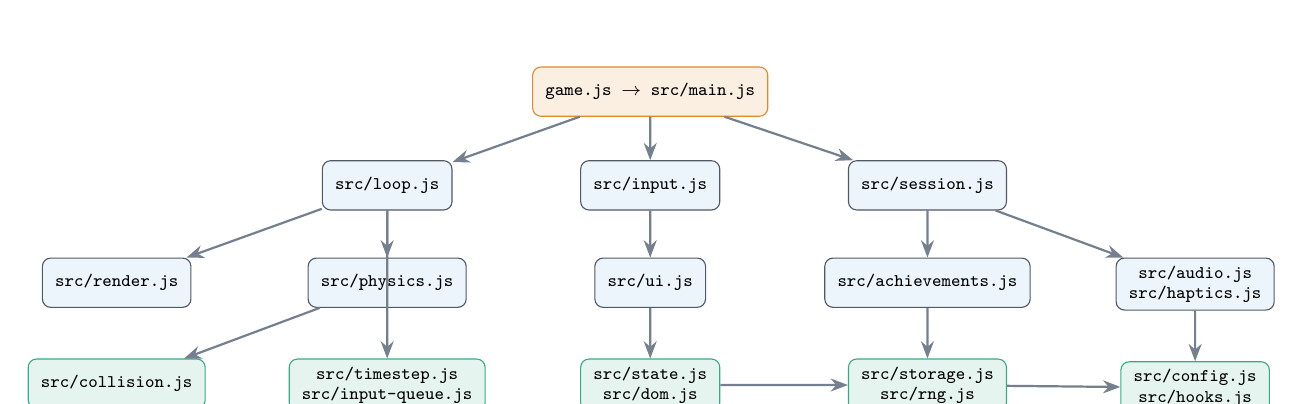
\begin{tikzpicture}[
  scale=0.92, transform shape,
  node distance=0.55cm and 0.45cm,
  tier/.style={rectangle, rounded corners=3pt, draw=gbNavy!70, fill=gbSky!8, minimum height=0.68cm, font=\scriptsize\ttfamily, align=center, inner xsep=5pt, inner ysep=3pt},
  pure/.style={tier, fill=gbEmerald!10, draw=gbEmerald!80},
  entry/.style={tier, fill=gbGold!12, draw=gbGold!85, font=\scriptsize\bfseries\ttfamily},
  arr/.style={-{Stealth[length=2.2mm]}, thick, draw=gbSlate!75}
]
  % Tier 0: Entry
  \node[entry] (entry) {game.js $\to$ src/main.js};

  % Tier 1: Orchestration
  \node[tier, below left=0.6cm and 1.1cm of entry] (loop) {src/loop.js};
  \node[tier, below=0.6cm of entry] (input) {src/input.js};
  \node[tier, below right=0.6cm and 1.1cm of entry] (session) {src/session.js};

  % Tier 2: Subsystems
  \node[tier, below left=0.65cm and 1.8cm of loop] (render) {src/render.js};
  \node[tier, below=0.65cm of loop] (physics) {src/physics.js};
  \node[tier, below=0.65cm of input] (ui) {src/ui.js};
  \node[tier, below=0.65cm of session] (ach) {src/achievements.js};
  \node[tier, below right=0.65cm and 1.5cm of session] (audio) {src/audio.js\\src/haptics.js};

  % Tier 3: Pure Formalized Core
  \node[pure, below=0.7cm of render] (coll) {src/collision.js};
  \node[pure, below=0.7cm of physics] (time) {src/timestep.js\\src/input-queue.js};
  \node[pure, below=0.7cm of ui] (state) {src/state.js\\src/dom.js};
  \node[pure, below=0.7cm of ach] (store) {src/storage.js\\src/rng.js};
  \node[pure, below=0.7cm of audio] (cfg) {src/config.js\\src/hooks.js};

  % Arrows
  \draw[arr] (entry) -- (loop);
  \draw[arr] (entry) -- (input);
  \draw[arr] (entry) -- (session);
  \draw[arr] (loop) -- (render);
  \draw[arr] (loop) -- (physics);
  \draw[arr] (input) -- (ui);
  \draw[arr] (session) -- (ach);
  \draw[arr] (session) -- (audio);
  \draw[arr] (physics) -- (coll);
  \draw[arr] (loop) -- (time);
  \draw[arr] (ui) -- (state);
  \draw[arr] (ach) -- (store);
  \draw[arr] (audio) -- (cfg);
  \draw[arr] (state) -- (store);
  \draw[arr] (store) -- (cfg);
\end{tikzpicture}
\caption{Acyclic five-tier native ES2022 module architecture of GlidieBirdie v3.2.0. Green boxes highlight pure algorithmic modules directly formalized in Lean~4.35.0 (\texttt{lean/GlidieBirdieProofs/}).}
\label{fig:arch}
\end{figure}

Three subtle cross-cutting architectural defects uncovered during our forensic hardening cycles warrant explicit documentation:
\begin{itemize}[leftmargin=1.6em, itemsep=1.5pt]
  \item \textbf{CSS Cascade Layer Inversion (\texttt{style.css}):} Under CSS Cascade Layers \cite{csslayers2022}, unlayered styles beat layered styles, and later layers beat earlier layers. Previously, \texttt{@media (prefers-\allowbreak reduced-\allowbreak transparency: reduce)} lived inside \texttt{@layer layout}, causing \texttt{@layer components} and unlayered \texttt{.toast} rules to override its opaque fallback backgrounds. Moving the media query unlayered to the end of \texttt{style.css} guarantees reduced-transparency overrides every panel, drawer, overlay, and toast.
  \item \textbf{Service Worker Cache-Key Shadowing (\texttt{service-worker.js}):} Query-parameterized requests (e.g.\ \texttt{./index.html?v=1}) previously checked \texttt{cache.\allowbreak match(request)} before normalized keys and left \texttt{cache.\allowbreak put()} unawaited inside background refresh. In v3.2.0, \texttt{stale\allowbreak While\allowbreak Revalidate()} looks up the normalized \texttt{cleanKey} first and awaits \texttt{cache.\allowbreak put(cleanKey, response.\allowbreak clone())} inside \texttt{event.\allowbreak waitUntil(networkFetch)}, ensuring refreshed shell assets always supersede legacy entries while caching all three PNG install icons (\texttt{180/192/512}).
  \item \textbf{Postcard Pose \& Game-Over Decay (\texttt{src/loop.js}, \texttt{src/render.js}):} \texttt{drawPostcard()} renders the interpolated pose inside \texttt{try/finally} without mutating simulation state; \texttt{afterglowTimer} decrements in seconds (\texttt{state.dtSec}) rather than frames; and \texttt{gameOver} decays shake and particles while freezing \texttt{state.time} under \texttt{prefers-\allowbreak reduced-\allowbreak motion}.
\end{itemize}

\section{Exact 720~Hz Fixed-Step Simulation and Input Quantization}
\label{sec:timestep}

Following Fiedler's fixed-timestep paradigm \cite{fiedler2004}, GlidieBirdie advances gameplay physics in exact $1/60\text{ s}$ steps (\texttt{SIM\_HZ = 60}) quantized onto a \texttt{TICK\_HZ = 720} integer tick grid (\texttt{src/timestep.js}). Converting wall-clock milliseconds $t_{\text{ms}}$ via
\begin{equation}
  \mathrm{msToTicks}(t_{\text{ms}}) = \mathrm{round}\!\left(\frac{18\, t_{\text{ms}}}{25}\right), \qquad \frac{720}{1000} = \frac{18}{25},
\end{equation}
with a finite guard ($\mathrm{msToTicks}(t) = 0$ if $t \notin \mathbb{R}$), aligns common display refresh rates exactly on integer tick multiples because $720 = \mathrm{lcm}(60, 144)$ and $720$ is divisible by $60, 120, 144, 240, 360,$ and $720$.

\begin{theorem}[60~Hz vs.\ 144~Hz Exact Step Parity \& Hitch Bounds --- \texttt{TimestepGrid.lean}]
\label{thm:timestep}
Set $\texttt{TICKS\_PER\_STEP} = 12$, $\texttt{TICKS\_PER\_144} = 5$, and $\texttt{MAX\_FRAME\_STEPS} = 5$. Then:
\begin{enumerate}[leftmargin=1.8em, itemsep=1pt]
  \item $\mathrm{lcm}(60, 144) = 720$, and $r \mid 720$ for every $r \in \{60, 120, 144, 240, 360, 720\}$.
  \item Over any $c \in \mathbb{N}$ cycles of $1/12\text{ s}$ ($60c$ ticks), a 60~Hz display ($5c$ frames) and a 144~Hz display ($12c$ frames) execute the exact same $5c$ simulation steps: $\lfloor (5c \cdot 12)/12 \rfloor = \lfloor (12c \cdot 5)/12 \rfloor = 5c$.
  \item For all $p, f \in \mathbb{N}$, $\mathrm{stepsExecuted}(p, f) \le 5$ is monotone in $f$ and equals $0$ when $f \le p$, while $\mathrm{alphaScaled}(f, s, b) \le 12$, guaranteeing $\alpha \in [0, 1]$ with zero hitch extrapolation. Moreover, whenever frame delta $\Delta t_{\text{ticks}} \le 60$ (all hitch-free refresh rates $\ge 12$~Hz, including 60~Hz and 144~Hz), $\mathrm{stepsExecuted}$ drops zero backlog (\texttt{steps\_executed\_no\_drop\_under\_60\_ticks}).
\end{enumerate}
\end{theorem}

All timestamped inputs (\texttt{flap}, \texttt{brake-on/off}, \texttt{dive-on/off}) enqueue in \texttt{src/input-queue.js} and fire on step boundaries \texttt{tick <= stepEndTick}. Cycle~1 auditing caught an off-by-one eviction guard (\texttt{queue.length > 64} allowed 65 entries) and missing \texttt{Number.\allowbreak isFinite(\allowbreak timeMs)} rejection (letting \texttt{NaN} ticks linger); both are hardened and proved in \texttt{PoolAndQueue.lean} (\texttt{queuePushMany\_\allowbreak bounded}).

\section{Euclidean Circle--Rectangle Collision and Universal Pipe Clearance}
\label{sec:collision}

GlidieBirdie replaces axis-aligned bounding-box (AABB) corner hits with exact circle-versus-rectangle distance testing \cite{ericson2004} in \texttt{src/collision.js}. Given circle $(c_x, c_y, c_r)$ and axis-aligned rectangle $[r_x, r_x+r_w] \times [r_y, r_y+r_h]$, the closest point $(q_x, q_y)$ is given by $q_x = \max(r_x, \min(c_x, r_x+r_w))$ and $q_y = \max(r_y, \min(c_y, r_y+r_h))$. Cycle~1 auditing found that unguarded $c_r < 0$ satisfies $d^2 < c_r^2$ since $(-|c_r|)^2 > 0$, while degenerate rectangles ($r_w \le 0$ or $r_h \le 0$) trigger phantom hits; v3.2.0 enforces $c_r > 0 \wedge r_w > 0 \wedge r_h > 0$ plus finiteness before clamping.

\begin{theorem}[Closest-Point Optimality \& Universal Pipe Clearance --- \texttt{CollisionGeometry.lean}]
\label{thm:collision}
Over exact integer coordinates:
\begin{enumerate}[leftmargin=1.8em, itemsep=1pt]
  \item \emph{Projection Optimality:} For every $(p_x, p_y) \in [r_x, r_x+r_w] \times [r_y, r_y+r_h]$,
  \[\mathrm{distSqPointRect}(c_x, c_y, r_x, r_y, r_w, r_h) \le (c_x - p_x)^2 + (c_y - p_y)^2.\]
  \item \emph{Soundness Guard:} Whenever $c_r \le 0 \vee r_w \le 0 \vee r_h \le 0$, $\mathrm{circleHitsRect} = \mathrm{false}$. Whenever $c_r, r_w, r_h > 0$ and $(c_x, c_y)$ lies inside the rectangle, $\mathrm{distSqPointRect} = 0$ and $\mathrm{circleHitsRect} = \mathrm{true}$.
  \item \emph{Universal Passability \& Conservative Radius Monotonicity:} With logical canvas $420 \times 640$, ground $y = 560$, pipe width $72$, gap $184$, and conservative bird radius $r = 18$, for every valid pipe height $h \in [60, 316]$ (covering the full moving-pipe oscillation range): $h + 184 < 560$, the gap exceeds $5\times$ the bird diameter ($184 > 180$), and a bird centered at $c_y = h + 92$ strictly misses both top and bottom pipes for every horizontal position $b_x, p_x \in \mathbb{Z}$. By \texttt{circleHitsRect\_\allowbreak monotone\_\allowbreak radius}, clearance at $r=18$ strictly implies clearance at every positive integer radius $1 \le r' \le 18$ (including $r'=15$, which conservatively bounds the forgiving runtime radius $0.82 \cdot 18 = 14.76$).
\end{enumerate}
\end{theorem}

\section{Object-Pool Conservation, Persistence Integrity, and Deterministic PRNG}
\label{sec:pools}

To prevent garbage-collection stalls during 60/144~Hz rendering, particles (\texttt{PARTICLE\_POOL = 220}) and weather flecks (\texttt{WEATHER\_POOL = 140}) use pre-allocated pools backed by explicit free-list index stacks (\texttt{freeParticles}, \texttt{freeWeather}), achieving $O(1)$ spawn and $O(1)$ reclamation. Previously, theme switching and reduced-motion toggles emptied \texttt{activeWeather.length = 0} without returning indices to \texttt{freeWeather}, permanently leaking capacity until weather stalled. Adding \texttt{clearWeatherPool()} restores every active index in $O(|\mathrm{activeWeather}|)$ time.

\begin{theorem}[Pool Conservation, Calendar Injectivity \& PRNG Parity]
\label{thm:pools}
The following invariants hold across \texttt{PoolAndQueue.lean}, \texttt{StorageStreak.lean}, and \texttt{PhysicsBounds.lean}:
\begin{enumerate}[leftmargin=1.8em, itemsep=1pt]
  \item \emph{Slot Conservation:} Under \texttt{poolInit}, \texttt{poolSpawn}, \texttt{poolReclaim}, and \texttt{poolClearAll}, $\mathrm{active} + \mathrm{free} = \mathrm{cap}$ holds inductively, $\mathrm{active} \le \mathrm{cap}$ universally, and \texttt{poolClearAll} sets $\mathrm{active} = 0$ and $\mathrm{free} = \mathrm{cap}$.
  \item \emph{Calendar Injectivity \& Streak Safety:} On all valid calendar triples $(y, m, d)$ with $1 \le m \le 12$ and $1 \le d \le 31$, $\mathrm{dateSeedNat}(y,m,d) = 10000y + 100m + d$ is strictly injective. Under \texttt{nextDayStreak}, same-day replays are idempotent, consecutive UTC days increment by $+1$, gaps reset to $1$, and the post-play streak is $\ge 1$ whenever $\mathrm{prevStreak} \ge 1 \vee \mathrm{lastDay} \neq \mathrm{today}$ (sharpness witnessed in \texttt{AdversarialTests.lean}).
  \item \emph{Difficulty Ramp, Shield Safety \& Exact PRNG:} The scaled speed multiplier $\mathrm{speedMult100}(s) = \min(118, 100 + 3\lfloor s/6 \rfloor)$ is monotone on $[100, 118]$, jumps at $s=6$, and saturates for all $s \ge 36$; active shields and invincibility never transition to \texttt{gameOver} on pipe impact; and the 32-bit \texttt{mulberry32Step} on daily seed \texttt{20261125} matches Node.js \texttt{src/rng.js} bit-for-bit across three consecutive outputs (\texttt{1176269751}, \texttt{1461114176}, \texttt{3047578727}).
\end{enumerate}
\end{theorem}

All persistent storage keys live under the \texttt{gb:} namespace (\texttt{STORAGE\_SCHEMA = '3'}) with one-time legacy migration, \texttt{QuotaExceededError}-safe wrappers, and allowlist filtering of both \texttt{THEMES} and \texttt{ACHIEVEMENT\_IDS} (hardened in Cycle~1 to block arbitrary injected achievement strings).

\section{Pure Lean~4.35.0 Multi-Kernel Verification and Statement Fidelity}
\label{sec:lean}

Following the Palomar Registry architecture \cite{palomar2026} and the Defensible Independent AI Research Playbook~(v1.3), the formal core under \texttt{lean/} uses Lean~\texttt{4.35.0} with \texttt{module} headers in every file, zero Mathlib or external Lake packages, and strict separation between \texttt{GlidieBirdieProofs/Spec.lean} (definitions only, zero proofs) and \texttt{Challenge.lean} (statement-only signatures) versus \texttt{Solution.lean} (sorry-free proofs).

\begin{table}[ht]
\centering
\caption{GlidieBirdie v3.2.0 Pure Lean~4.35.0 Formal Verification Summary (68 Theorems, Zero Mathlib).}
\label{tab:lean}
\footnotesize
\setlength{\tabcolsep}{4pt}
\begin{tabular}{@{} l r >{\raggedright\arraybackslash}p{6.0cm} >{\raggedright\arraybackslash}p{4.3cm} @{}}
\toprule
\textbf{Module} & \textbf{Thms} & \textbf{Axioms Used (Max Set)} & \textbf{Runtime Source Anchors} \\
\midrule
\texttt{TimestepGrid.lean} & 13 & \texttt{[propext, Classical.choice, Quot.sound]} (4 zero-axiom) & \texttt{src/timestep.js}, \texttt{src/loop.js} \\
\texttt{CollisionGeometry.lean} & 9 & \texttt{[propext, Classical.choice, Quot.sound]} & \texttt{src/collision.js}, \texttt{src/config.js} \\
\texttt{StorageStreak.lean} & 8 & \texttt{[propext, Classical.choice, Quot.sound]} & \texttt{src/storage.js}, \texttt{src/rng.js} \\
\texttt{PoolAndQueue.lean} & 13 & \texttt{[propext, Classical.choice, Quot.sound]} (1 zero-axiom) & \texttt{src/physics.js}, \texttt{src/input-queue.js} \\
\texttt{PhysicsBounds.lean} & 11 & \texttt{[propext, Classical.choice, Quot.sound]} (3 zero-axiom) & \texttt{src/physics.js}, \texttt{src/rng.js} \\
\texttt{NonVacuity.lean} & 5 & \texttt{[propext, Classical.choice, Quot.sound]} (3 zero-axiom) & Concrete realizability witnesses \\
\texttt{AdversarialTests.lean} & 9 & \texttt{[propext, Quot.sound]} (8 zero-axiom) & Constructive false-variant refutations \\
\midrule
\textbf{Total} & \textbf{68} & \textbf{19 zero-axiom; zero \texttt{sorryAx}, zero \texttt{native\_decide}, zero custom axioms} & \textbf{6-kernel \texttt{lake comparator --paranoid} + live negative tamper} \\
\bottomrule
\end{tabular}
\end{table}

\subsection{Statement-Fidelity Audit (Honest Formal-to-Runtime Boundary)}
A formal proof is only as meaningful as the fidelity between its Lean definitions and the shipped JavaScript implementation. Table~\ref{tab:fidelity} audits each formalized abstraction against \texttt{src/} and states the exact modeling boundary explicitly.

\begin{table}[ht]
\centering
\caption{Statement-Fidelity Audit: Lean~4 Declarations vs.\ Shipped ES2022 Runtime (\texttt{src/}).}
\label{tab:fidelity}
\footnotesize
\setlength{\tabcolsep}{4pt}
\begin{tabular}{@{} >{\raggedright\arraybackslash}p{3.8cm} >{\raggedright\arraybackslash}p{3.4cm} >{\raggedright\arraybackslash}p{5.0cm} c @{}}
\toprule
\textbf{Lean Declaration} & \textbf{Runtime Symbol} & \textbf{Exact Fidelity Notes \& Gap} & \textbf{Status} \\
\midrule
\texttt{stepsExecuted}, \texttt{alphaScaled}, \texttt{shouldContinueLoop} & \texttt{src/timestep.js}, \texttt{src/loop.js} & Exact integer division matches \texttt{Math.floor(tick / 12)}, \texttt{MAX\_FRAME\_STEPS = 5}, 252-step afterglow, and idle sleep predicate; JS \texttt{msToTicks} rounds IEEE-754 float \texttt{ms} first. & \textbf{Exact (grid)} \\
\texttt{distSqPointRect}, \texttt{circleHitsRect}, \texttt{intersectsPipeInt} & \texttt{src/collision.js} & Exact algebraic match over $\mathbb{Z}$; runtime uses float64 and shrunken $0.82\cdot 18=14.76$ radius, bridged conservatively by \texttt{circleHitsRect\_\allowbreak monotone\_\allowbreak radius} + 1,000-trial \texttt{prop\_check}. & \textbf{Conservative} \\
\texttt{nextDayStreak}, \texttt{dateSeedNat}, \texttt{clampIntBounds} & \texttt{src/storage.js}, \texttt{src/rng.js} & Exact 1-to-1 logic; JS also guards \texttt{NaN}/non-finite bounds before comparison (verified by 1,500 parser fuzz cases). & \textbf{Exact} \\
\texttt{PoolState}, \texttt{ListPool}, \texttt{fifoPush} & \texttt{src/physics.js}, \texttt{src/input-queue.js} & Certifies both slot cardinality and concrete \texttt{Nodup} index disjointness + bounded FIFO list length; mutable JS array fields verified by \texttt{engine-test.mjs}, $5\times 10$k churn, and 1M C11 fuzz cases. & \textbf{Concrete list} \\
\texttt{speedMult100}, \texttt{mulberry32Step}, \texttt{lerpPipeTopScaled} & \texttt{src/physics.js}, \texttt{src/rng.js} & \texttt{mulberry32Step} matches JS and C11 bit-for-bit; \texttt{speedMult100}, sclera gaze bound, and moving-pipe lerp scale exact integer bounds. & \textbf{Bit-exact PRNG} \\
\bottomrule
\end{tabular}
\end{table}

\section{Empirical Verification, Fuzzing, Mutation, and Benchmarks}
\label{sec:eval}

Formal proofs establish specification soundness; empirical verification tests the actual JavaScript runtime, DOM accessibility, and HTTP server under adversarial conditions.

\subsection{Paired 60~Hz vs.\ 144~Hz Determinism and Performance Benchmarks}
We executed \texttt{node scripts/benchmark.mjs} on an \texttt{Intel Core Ultra 9 275HX} (24 cores, Windows \texttt{10.0.29704} x64, \texttt{Node v25.8.2}, default V8 flags) with 5 untimed warmup seeds followed by \textbf{30 counterbalanced paired seeds} (\texttt{20261101}--\texttt{20261130}; even seeds run $60\to 144$~Hz, odd seeds run $144\to 60$~Hz), each executing 180 fixed 60~Hz steps (3.0~s hitch-free gameplay) on the 720~Hz tick grid against a naive variable-$\Delta t$ Euler baseline. Pure simulation timing isolates \texttt{stepSimulation()} directly across all 5,400 individual steps; whole-loop timing separately reports amortized per-seed averages including headless \texttt{present()}/\texttt{draw()}. Raw per-seed observations are published in \texttt{results/benchmarks.json}; multiple comparisons use Holm--Bonferroni \cite{holm1979}.

\begin{table}[ht]
\centering
\caption{Counterbalanced 30-Seed Determinism, Pure-Step Latency, and Pool-Churn Benchmarks (\texttt{benchmarks.json}).}
\label{tab:bench}
\scriptsize
\setlength{\tabcolsep}{3.5pt}
\begin{tabular}{@{} l r r r r @{}}
\toprule
\textbf{Metric ($N=30$ seeds; $5{,}400$ pure steps)} & \textbf{60~Hz Fixed} & \textbf{Comparison / Budget} & \textbf{Wins} & \textbf{$p_{\text{Holm}}$} \\
\midrule
Max 60~Hz vs.\ 144~Hz vertical drift (px) & \textbf{0.000} & Naive: 4.783 & 30/30 & $3.73\times 10^{-9}$ \\
Median 60~Hz vs.\ 144~Hz vertical drift (px) & \textbf{0.000} & Naive: 3.855 & --- & --- \\
Mean drift $\pm$ 95\% CI (px) & \textbf{0.000 $[0, 0]$} & $3.944\;[3.820, 4.069]$ & --- & --- \\
Pure sim individual step: med / p95 / max ($\mu$s) & \textbf{0.50 / 2.10 / 316.40} & Budget: 16,666.67 (0 viol.) & 30/30 & $3.73\times 10^{-9}$ \\
Amortized whole-loop (incl.\ draw): 60 / 144~Hz ($\mu$s) & \textbf{3.92 / 10.31} (med) & p95: 10.15 / 13.14 (30 runs) & --- & --- \\
10,000-cycle pool churn ($5$ reps): med / 95\% CI & \textbf{17.02~ms $[15.47, 19.62]$} & \textbf{1.70~$\mu$s/cycle}, 0 viol. & --- & --- \\
\bottomrule
\end{tabular}
\end{table}

\begin{figure}[ht]
\centering
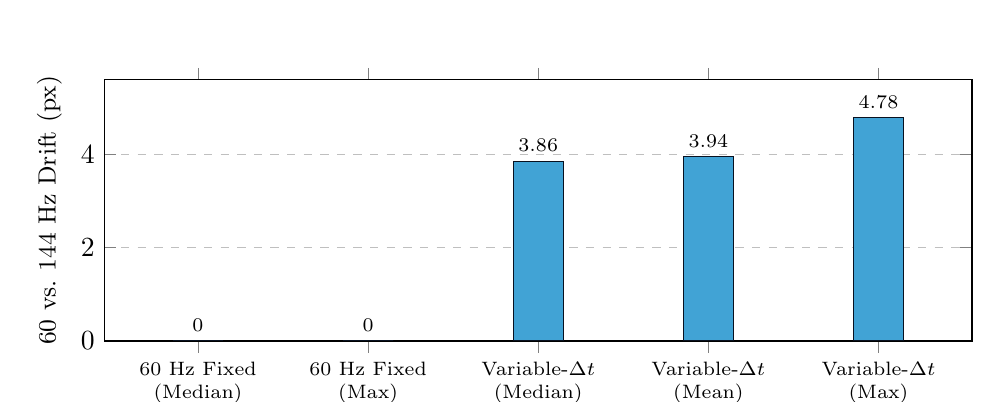
\begin{tikzpicture}
\begin{axis}[
  ybar,
  width=12.6cm,
  height=4.9cm,
  bar width=18pt,
  ylabel={60 vs.\ 144~Hz Drift (px)},
  ylabel style={font=\small},
  xtick={1,2,3,4,5},
  xticklabels={
    {60~Hz Fixed\\(Median)},
    {60~Hz Fixed\\(Max)},
    {Variable-$\Delta t$\\(Median)},
    {Variable-$\Delta t$\\(Mean)},
    {Variable-$\Delta t$\\(Max)}
  },
  xticklabel style={font=\scriptsize, align=center},
  ymin=0, ymax=5.6,
  xmin=0.45, xmax=5.55,
  nodes near coords,
  nodes near coords style={font=\scriptsize\bfseries},
  ymajorgrids=true,
  grid style=dashed
]
\addplot[fill=gbSky!75, draw=gbNavy] coordinates {
  (1, 0.000)
  (2, 0.000)
  (3, 3.855)
  (4, 3.944)
  (5, 4.783)
};
\end{axis}
\end{tikzpicture}
\caption{Measured 60~Hz vs.\ 144~Hz maximum vertical trajectory drift across 30 counterbalanced paired seeds (\texttt{results/benchmarks.json}). GlidieBirdie's 60~Hz fixed-step loop on a 720~Hz integer tick grid achieves exact 0.000~px divergence.}
\label{fig:drift}
\end{figure}

\subsection{Property Testing, Adversarial Fuzzing, and Surgical Mutation}
To eliminate false confidence from hand-picked unit examples, GlidieBirdie pairs QuickCheck-style property testing \cite{claessen2000} and metamorphic invariance checks \cite{chen2018} (\texttt{tests/\allowbreak property-\allowbreak and-\allowbreak metamorphic.mjs}) with a 2,000-case structured adversarial fuzzer (\texttt{tests/\allowbreak fuzz-\allowbreak http-\allowbreak and-\allowbreak inputs.mjs}: 1,500 parser/engine cases + 500 HTTP static-server cases) and baseline-gated surgical single-line mutation testing \cite{jia2011} (\texttt{scripts/\allowbreak mutation-\allowbreak test.mjs}). Both adversarial harnesses paid immediate dividends:
\begin{itemize}[leftmargin=1.6em, itemsep=1.5pt]
  \item \textbf{Mutation Holes \texttt{M03}, \texttt{M09} \& Thermal/Visual Guards \texttt{M13}--\texttt{M16}:} Initial mutation testing caught that \texttt{tests/\allowbreak determinism.mjs} omitted \texttt{a.length === 180} (letting corrupted \texttt{TICKS\_\allowbreak PER\_\allowbreak STEP = 10} run 20\% fast) and \texttt{tests/\allowbreak engine-\allowbreak test.mjs} omitted mid-run paused \texttt{resetStats()}. Expanding to 16 mutants (adding identical-DPR resize guard \texttt{M13}, paused idle sleep \texttt{M14}, sclera pupil clamp \texttt{M15}, and \texttt{AudioContext.suspend()} power-gating \texttt{M16}) raised coverage to \textbf{16/16 (100.0\%)} with baseline validation and runner-error separation.
  \item \textbf{Fuzzer (\texttt{F16}--\texttt{F17}) \& Offline C11 Oracle:} The 2,000-case JS fuzzer exposed \texttt{clamp\allowbreak Number()} returning \texttt{NaN}/\texttt{Infinity} on non-finite bounds (\texttt{F16}) and WHATWG \texttt{new URL()} collapsing \texttt{/\%2e\%2e/\allowbreak .env/\allowbreak ../\allowbreak \%2e\%2e} to \texttt{/} (\texttt{F17}). An offline ISO~C11 reference oracle (\texttt{native/\allowbreak glidiebirdie\_\allowbreak oracle.c}, built with \texttt{-std=c11 -O3 -Wall -Wextra -Werror} and ASan/\allowbreak UBSan in CI) independently verifies bit-for-bit parity with JS and Lean~4 plus 1,000,000 fuzz iterations; empirical profiling (\texttt{results/\allowbreak native-\allowbreak comparison.json}, \texttt{results/\allowbreak browser-\allowbreak thermal.json}) confirms V8 runs the collision kernel at 16.09~ns/iter (faster than per-call Zig--WASM at 26.58~ns/iter) while demand-driven sleep drops paused rendering to \textbf{0.0~FPS} (ADR~0004).
\end{itemize}

\begin{table}[ht]
\centering
\caption{Baseline-Gated Surgical Mutation Kill Matrix (\texttt{scripts/mutation-test.mjs}: 16/16 = 100.0\% Killed).}
\label{tab:mutants}
\footnotesize
\setlength{\tabcolsep}{4pt}
\begin{tabular}{@{} c l >{\raggedright\arraybackslash}p{6.5cm} l c @{}}
\toprule
\textbf{ID} & \textbf{Module} & \textbf{Planted Defect} & \textbf{Killing Suite} & \textbf{Status} \\
\midrule
\texttt{M01} & \texttt{src/collision.js} & Drop non-positive radius guard (\texttt{!(cr > 0)}) & \texttt{property-and-metamorphic} & \textbf{KILLED} \\
\texttt{M02} & \texttt{src/collision.js} & Invert distance inequality (\texttt{<} $\to$ \texttt{>}) & \texttt{engine-test.mjs} & \textbf{KILLED} \\
\texttt{M03} & \texttt{src/timestep.js} & Corrupt \texttt{TICKS\_PER\_STEP} ($12 \to 10$) & \texttt{determinism.mjs} & \textbf{KILLED} \\
\texttt{M04} & \texttt{src/storage.js} & Corrupt streak increment ($+1 \to +2$) & \texttt{engine-test.mjs} & \textbf{KILLED} \\
\texttt{M05} & \texttt{src/storage.js} & Remove \texttt{ACHIEVEMENT\_IDS} allowlist & \texttt{property-and-metamorphic} & \textbf{KILLED} \\
\texttt{M06} & \texttt{src/input-queue.js} & Relax 64-slot FIFO eviction cap & \texttt{property-and-metamorphic} & \textbf{KILLED} \\
\texttt{M07} & \texttt{src/physics.js} & Re-introduce \texttt{clearWeatherPool} leak & \texttt{engine-test.mjs} & \textbf{KILLED} \\
\texttt{M08} & \texttt{src/loop.js} & Re-introduce \texttt{afterglowTimer} frame-unit bug & \texttt{engine-test.mjs} & \textbf{KILLED} \\
\texttt{M09} & \texttt{src/achievements.js} & Re-introduce mid-run \texttt{resetStats} re-grant & \texttt{engine-test.mjs} & \textbf{KILLED} \\
\texttt{M10} & \texttt{src/audio.js} & Disable zero-volume \texttt{playToneAt} guard & \texttt{engine-test.mjs} & \textbf{KILLED} \\
\texttt{M11} & \texttt{tools/static-server} & Disable public static asset allowlist & \texttt{property-and-metamorphic} & \textbf{KILLED} \\
\texttt{M12} & \texttt{src/timestep.js} & Remove \texttt{msToTicks} non-finite guard & \texttt{property-and-metamorphic} & \textbf{KILLED} \\
\texttt{M13} & \texttt{src/dom.js} & Disable identical-DPR resize rebuild guard & \texttt{engine-test.mjs} & \textbf{KILLED} \\
\texttt{M14} & \texttt{src/loop.js} & Force \texttt{shouldContinueLoop()} spin while paused & \texttt{engine-test.mjs} & \textbf{KILLED} \\
\texttt{M15} & \texttt{src/physics.js} & Re-introduce detached pupil \texttt{lookX = 18} bug & \texttt{engine-test.mjs} & \textbf{KILLED} \\
\texttt{M16} & \texttt{src/audio.js} & Disable \texttt{AudioContext.suspend()} power-gating & \texttt{engine-test.mjs} & \textbf{KILLED} \\
\bottomrule
\end{tabular}
\end{table}

Browser-level verification runs 7 Playwright + axe-core end-to-end tests in Chromium (\texttt{tests/\allowbreak e2e/\allowbreak smoke.spec.js}) validating keyboard flight and pause, modal focus trapping, tutorial shortcut blocking, Serene Postcard \texttt{P}/\texttt{Escape}/\texttt{R} lifecycle, live \texttt{ThemeExplorer} unlock with \texttt{page.\allowbreak reload()} persistence, \texttt{prefers-\allowbreak reduced-\allowbreak motion}, and zero automated WCAG~2.2~AA violations across all four interactive views (initial playfield, Customizer drawer, Tutorial modal, and Serene Postcard).

\section{Threat Model, Limitations, Epistemic Scope, and AI Disclosure}
\label{sec:limits}

\subsection{Security Surface and Limitations}
GlidieBirdie stores only non-sensitive gameplay preferences and high scores locally via \texttt{localStorage} and makes zero outbound network calls. Its primary security boundaries are: (1)~strict Content-Security-Policy (\texttt{default-src 'self'}) in \texttt{index.html} (noting that \texttt{frame-ancestors} is header-only and cannot be enforced via \texttt{<meta>} on GitHub Pages); (2)~corrupted or tampered \texttt{localStorage} inputs (mitigated by finite-bound-safe clamping, JSON try/catch recovery, and \texttt{THEMES}/\allowbreak\texttt{ACHIEVEMENT\_IDS} allowlists); and (3)~the local development server \texttt{tools/static-server.mjs} (mitigated by a strict public static allowlist blocking \texttt{.git/}, \texttt{.env}, \texttt{package.json}, \texttt{tools/}, and \texttt{tests/}, raw-URL pre-normalization dot-segment rejection, IPv6-safe URL parsing, \texttt{realpath} symlink confinement, \texttt{405} non-GET/HEAD rejection, and \texttt{nosniff}/\allowbreak\texttt{X-Frame-Options: DENY} headers).

Key engineering limitations (detailed in \texttt{LIMITATIONS.md}):
\begin{enumerate}[leftmargin=1.8em, itemsep=1pt]
  \item Native ES modules require HTTP/HTTPS serving; opening \texttt{index.html} directly via \texttt{file://} is blocked by browser CORS policy.
  \item Lean~4 proofs cover exact discrete integer/\texttt{UInt32} models rather than IEEE-754 floating-point canvas rendering or browser Web Audio DSP internals; automated axe-core scans complement rather than replace manual assistive-technology audits.
  \item Local browser persistence (\texttt{localStorage}) is client-controlled and not tamper-proof against a user modifying DevTools storage directly; no leaderboard integrity is claimed.
\end{enumerate}

\subsection{Unsolved Problems Mega-Atlas Scope and AI-Assistance Disclosure}
\textbf{Mega-Atlas Audit:} Audited explicitly against the 1,900 open problems cataloged in \texttt{0thernes/\allowbreak unsolved-\allowbreak problems-\allowbreak mega-\allowbreak atlas} (v2.6.0), GlidieBirdie retires \textbf{0 / 1,900} open problems. It is a verified interactive software engineering system, not a mathematical conjecture proof.

\textbf{AI-Assistance and Provenance Disclosure:} This repository, its formal Lean~4 proofs, test suites, and technical white paper were developed by Alexander Stephen Donahue with substantial AI engineering assistance (Antigravity/Gemini, Claude, and Codex across versions v2.0--v3.2). No peer review, journal acceptance, arXiv endorsement, or external DOI is claimed. Independent soundness rests strictly on reproducible mechanical verification: the Lean~4.35.0 kernel and 6-kernel comparator (68 theorems + live negative tamper check), 81 engine tests, 8 property/metamorphic/HTTP allowlist suites, 2,000 JS + 1,000,000 C11 differential oracle fuzz cases (with ASan/UBSan in CI), 16/16 baseline-gated mutation tests, 12/12 citation checks, 7 Playwright + 4-view axe-core WCAG~2.2~AA tests, and deterministic SHA-256 build artifacts.

\FloatBarrier
\bibliographystyle{plain}
\bibliography{references}

\end{document}
